\documentclass[pdftex,12pt,a4paper]{article}

\usepackage{graphicx}  
\usepackage[margin=2.5cm]{geometry}
\usepackage{breakcites}
\usepackage{indentfirst}
\usepackage{pgfgantt}
\usepackage{pdflscape}
\usepackage{float}
\usepackage{epsfig}
\usepackage{epstopdf}
\usepackage[cmex10]{amsmath}
\usepackage{stfloats}
\usepackage{multirow}

\renewcommand{\refname}{REFERENCES}
\linespread{1.3}

\usepackage{mathtools}
%\newcommand{\HRule}{\rule{\linewidth}{0.5mm}}
\thispagestyle{empty}
\begin{document}
\begin{titlepage}
\begin{center}
\textbf{}\\
\textbf{\Large{ISTANBUL TECHNICAL UNIVERSITY}}\\
\vspace{0.5cm}
\textbf{\Large{COMPUTER ENGINEERING DEPARTMENT}}\\
\vspace{2cm}
\textbf{\Large{BLG 242E\\ DIGITAL CIRCUITS LABORATORY\\ EXPERIMENT REPORT}}\\
\vspace{2.8cm}
\begin{table}[ht]
\centering
\Large{
\begin{tabular}{lcl}
\textbf{EXPERIMENT NO}  & : & 6 \\
\textbf{EXPERIMENT DATE}  & : & 22.03.2019 \\
\textbf{LAB SESSION}  & : & FRIDAY - 14.00 \\
\textbf{GROUP NO}  & : & G13 \\
\end{tabular}}
\end{table}
\vspace{1cm}
\textbf{\Large{GROUP MEMBERS:}}\\
\begin{table}[ht]
\centering
\Large{
\begin{tabular}{rcl}
{
150180704  & : & C\.{I}HAT AKK\.{I}RAZ \\
150180707  & : & FAT\.{I}H ALTINPINAR \\
150180734  & : & S\.{I}NAN \c{S}AR \\
}
\end{tabular}}
\end{table}
\vspace{2.8cm}
\textbf{\Large{SPRING 2019}}

\end{center}

\end{titlepage}

\newpage

\thispagestyle{empty}
\centering{\LARGE{ \textbf{ETHIC FORM}}}\\
\centering{\LARGE{\textbf{for}}}\\
\centering{\LARGE{\textbf{BLG242E Logic Circuits Laboratory}}}\\[0.2cm]
As a student of \\Istanbul Technical University Faculty of Computer and Informatics Engineering;
\begin{enumerate}
    \item I will not attempt to cheat in quizes and final exam,
    \item I will not use disallowed sources or tools (mobile phone, calculator etc.) during the exam,
    \item I will not write any information (formula, text, figure etc.) on the table, sheets or books that are allowed to be used during the exam,
    \item I will give reference when using printed or online published sources,
    \item I will not use the results in a source as they are, or by changing a part of them without giving a reference,
    \item I will not show unused sources as used, 
    \item I will not present someone else’s idea as my own idea, 
    \item I will not make someone do my homework, project or thesis for money or anything else,
    \item I will not take an exam or enter a lecture on behalf of others,
    \item I will not make excuses for not attending in exams or lessons by taking reports from someone I know (medical doctor parents or relatives),
    \item I will refrain from deliberately harming the public materials at our university,  
    \item I will comply with the safety rules in laboratory work,
    \item I will behave in accordance with the rules of respect for the lecturers and teaching assistants
\end{enumerate}
\vspace{-1em}
\centering{\LARGE{signed by}}\\
\vspace{-1em}
\begin{table}[ht]
\centering
\begin{tabular}{rcl}
150180704  & : & C\.{I}HAT AKK\.{I}RAZ \\
150180707  & : & FAT\.{I}H ALTINPINAR \\
150180734  & : & S\.{I}NAN \c{S}AR \\
\end{tabular}
\end{table}
\vspace{-1em}
 \begin{table}[ht]
 \begin{tabular}{lr}
%\textbf{Date:\hspace*{1.0cm}/\hspace*{1.0cm}/} &\qquad \qquad\qquad\qquad \qquad\qquad\qquad \qquad\qquad\qquad \qquad\qquad \textbf{SIGNED}\\
\end{tabular}
\end{table} % adds the ethic sign
\addcontentsline{toc}{section}{\numberline {}ETHICS}
\newpage

\thispagestyle{empty}
\addtocontents{toc}{\contentsline {section}{\numberline {}FRONT COVER}{}}
\addtocontents{toc}{\contentsline {section}{\numberline {}CONTENTS}{}}
\setcounter{tocdepth}{4}
\tableofcontents
\clearpage

\setcounter{page}{1}

\section{INTRODUCTION}
\begin{flushleft}
\paragraph{}
In this experiment, a data bus is implemented by using three-state buffers and ICs with open collector outputs. Main goal is understanding the behavior of a data bus and its basic principles. 
\end{flushleft}
\section{REQUIREMENTS}
\begin{flushleft}
\underline{Tools Used}\cite{booklet}
\end{flushleft}

\begin{itemize}
    \item C.A.D.E.T
    \item 74000 series ICs
    \begin{itemize}
        \item 74xx241 Octal 3-State Buffer
        \item 74xx05 Hex Inverters with Open-Collector Outputs 
    \end{itemize}
    \item Resistors
    \item 100$\Omega$ Resistor
\end{itemize}

\begin{flushleft}
\subsection{PART 1}

\paragraph{}
In the first part of the experiment, 4-bit data bus is implemented by using ICs with given outputs(given Hex Inverters with open collectors). $R_{C(max)}$ and $R_{C(min)}$ values are calculated for $V_{cc)}$=5.0V, N=1, K=2, $V_{IL(max)}$=0.8V, $V_{IH(min)}$=2.0V, $I_{IL(max)}$=0.4mA, $I_{OL(max)}$=8mA, $I_{OH(max)}$=100$\mu$A,  $I_{IH(max)}$=20$\mu$A as given formulas. Resistances were used according to the results of the calculations. 



\begin{itemize}
    \item $R_{C(min)}$ = [$V_{cc}$ - $V_{IL(max)}$]/[$I_{OL(max)}$-$I_{IL(max)}$ $\cdot$ N]
    \item $R_{C(max)}$ = [$V_{cc}$ - $V_{IH(min)}$]/[$I_{OH(max)}$ $\cdot$ K + $I_{IH(max)}$ $\cdot$ N]
\end{itemize}

\paragraph{}    
When calculation is completed $R_{C(min)}$ and $R_{C(max)}$ values are found as 0.552k$\Omega$ and 13,636k$\Omega$. In this experiment 4.7k$\Omega$ resistances are used suitability of the resistance value validated with the calculations.

\begin{figure}[h]
	\centering
	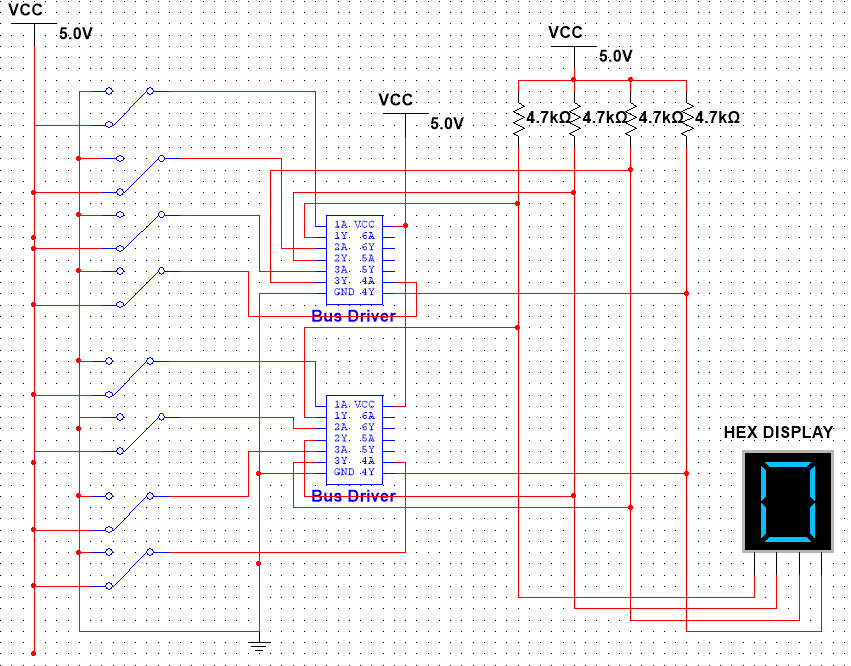
\includegraphics[width=0.7\textwidth]{part1.png}	
	\caption{4 bit data bus with 2 drivers with open collector outputs}
	\label{circ:part1}
\end{figure}

\paragraph{}
Inputs are connected from logic switches to Octal 3-State Buffer. Output pins of Octal 3-State Buffer are inverted by using hex inverter. Output pins of hex inverters are connected to displays and results are observed as given circuit below. Results are validated with the information that bus behaves like a 'wired or' circuit.

\begin{table}[h]
\centering
\begin{tabular}{|l|l|l|}
\hline
1Ax & 2Ax & Yx \\ \hline
1   & 1   & 0  \\ \hline
1   & 0   & 0  \\ \hline
0   & 1   & 0  \\ \hline
0   & 0   & 1  \\ \hline
\end{tabular}
\label{table:part1}
\caption{Results of Part 1}
\end{table}




\end{flushleft}

\begin{flushleft}
\subsection{PART 2}

\paragraph{}
In the second part of the experiment, 4-bit bus is implemented by using 3 state buffers. One of the SPDT switches is used for enable input of the 3 state buffers as given in circuit figure below. After the implementation, result is observed on the display. Behaviour of the circuit seems in the table below.

\begin{table}[]
    \centering
    \begin{tabular}{|c|c|c|c|}
        \hline
         SPDT & A1   & A2   & Y \\ \hline
         H    & 0xC  & 0xB  & 0xB \\ \hline
         H    & 0x09  & 0x07  & 0x07 \\ \hline
         L    & 0xA  & 0xC  & 0xA \\ \hline
         L    & 0x03  & 0xE  & 0x03 \\ \hline
    \end{tabular}
    \caption{3 state buffers with SPDT switches}
    \label{tab:my_label}
\end{table}

\begin{figure}[h]
	\centering
	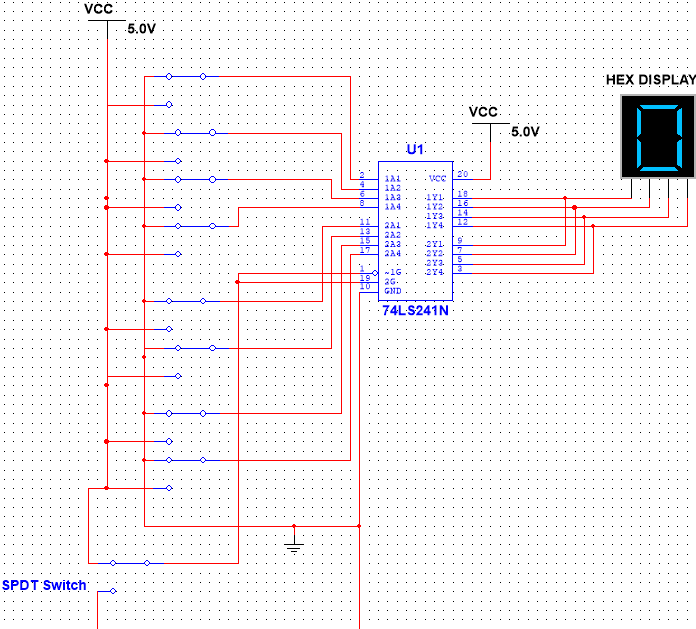
\includegraphics[width=0.5\textwidth]{part2.png}	
	\caption{4 bit data bus with 2 drivers with 3-state buffers}
	\label{circ:part2}
\end{figure}
\end{flushleft}


\newpage
\begin{flushleft}
\subsection{PART 3}

\paragraph{}
In the final part of the experiment, the circuit is implemented as in the figure given below. The circuit contains 2-bit bus with two distinct outputs and inputs. One of the SPDT switches is used for enable input of the 3-state buffers.

\paragraph{}
Behaviour of the bus is validated according to the results observed on the LED outputs. Then, SPDT switch connection is detached and connected to the frequency generator instead of enable pin. Output of the circuit is observed changing frequency. Behaviour of the circuit is seems on the table below.


\end{flushleft}

\begin{figure}[!h]
	\centering
	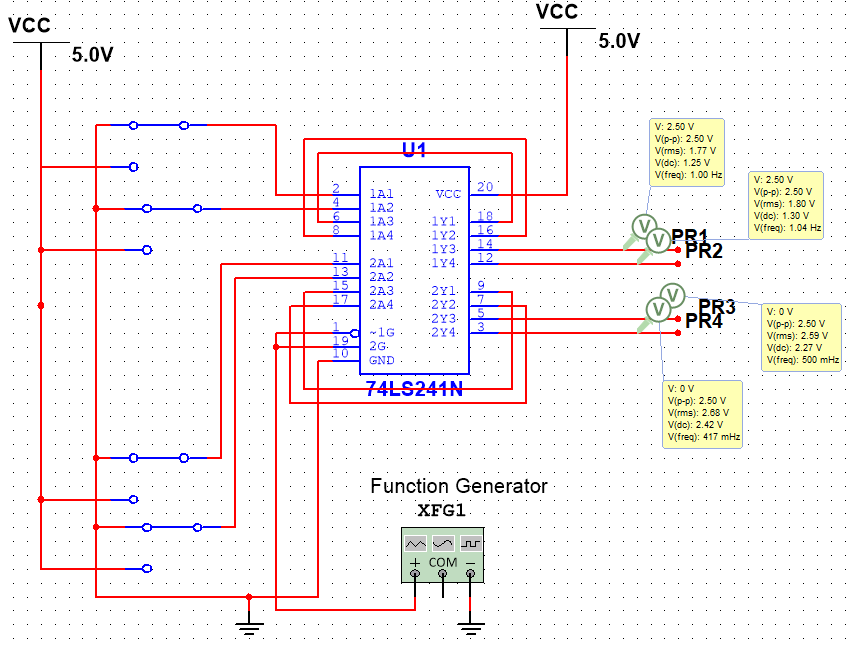
\includegraphics[width=0.5\textwidth]{part3.png}	
	\caption{2 bit data bus with 2 drivers and 2 readers}
	\label{circ:part3}
\end{figure}


\begin{table}[!h]
\centering
\begin{tabular}{|c|c|c|c|c|c|c|c|c|c|c|c|}
\hline
\multicolumn{6}{|c|}{While CLK is High} & \multicolumn{6}{c|}{While CLK is Low} \\ \hline
1A1   & 1A2   & 2A1  & 2A2  & Y1  & Y2  & 1A1  & 1A2  & 2A1  & 2A2  & Y1  & Y2  \\ \hline
0     & 0     & 0    & 0    & 0   & 0   & 0    & 0    & 0    & 0    & 0   & 0   \\ \hline
0     & 0     & 0    & 1    & 0   & 1   & 0    & 0    & 0    & 1    & 0   & 0   \\ \hline
0     & 0     & 1    & 0    & 1   & 0   & 0    & 0    & 1    & 0    & 0   & 0   \\ \hline
0     & 0     & 1    & 1    & 1   & 1   & 0    & 0    & 1    & 1    & 0   & 0   \\ \hline
0     & 1     & 0    & 0    & 0   & 0   & 0    & 1    & 0    & 0    & 0   & 1   \\ \hline
0     & 1     & 0    & 1    & 0   & 1   & 0    & 1    & 0    & 1    & 0   & 1   \\ \hline
0     & 1     & 1    & 0    & 1   & 0   & 0    & 1    & 1    & 0    & 0   & 1   \\ \hline
0     & 1     & 1    & 1    & 1   & 1   & 0    & 1    & 1    & 1    & 0   & 1   \\ \hline
1     & 0     & 0    & 0    & 0   & 0   & 1    & 0    & 0    & 0    & 1   & 0   \\ \hline
1     & 0     & 0    & 1    & 0   & 1   & 1    & 0    & 0    & 1    & 1   & 0   \\ \hline
1     & 0     & 1    & 0    & 1   & 0   & 1    & 0    & 1    & 0    & 1   & 0   \\ \hline
1     & 0     & 1    & 1    & 1   & 1   & 1    & 0    & 1    & 1    & 1   & 0   \\ \hline
1     & 1     & 0    & 0    & 0   & 0   & 1    & 1    & 0    & 0    & 1   & 1   \\ \hline
1     & 1     & 0    & 1    & 0   & 1   & 1    & 1    & 0    & 1    & 1   & 1   \\ \hline
1     & 1     & 1    & 0    & 1   & 0   & 1    & 1    & 1    & 0    & 1   & 1   \\ \hline
1     & 1     & 1    & 1    & 1   & 1   & 1    & 1    & 1    & 1    & 1   & 1   \\ \hline
\end{tabular}
\label{table:part3}
\caption{Results recorded in part3}
\end{table}

\newpage


\section{INTERPRETATION OF THE RESULTS}
Results throughout the whole experiment were consistent with the results we have calculated beforehand. Bus behaved as we expected in all off the circuits that were implemented.
\section{CONCLUSION}
Everything went as planned through the whole experiment, we did not have any difficulties completing the given tasks. All in all, we believe that this experiment helped us improve our knowledge of implementations of BUS.

\nocite{overleaf}
\nocite{reportGuide}

\newpage
\addcontentsline{toc}{section}{\numberline {}REFERENCES}

\bibliographystyle{unsrt}
\bibliography{reference}

\end{document}

